\section{Minimum bias data}

To minimise the bias of data from inelastic collisions collected from collider experiments, experimentalists use a trigger with a minimal set of criteria - generally called the minimum bias trigger. This trigger will typical involve requirements such as a minimum number of hits in an event or an event with at least one reconstructed track. Biases are still present due to collisions that are not detectable such as collisions that result in  particles with trajectories collinear to the initial trajectory of the beam particles; these particles continue along the beam pipe leaving no sign in the sensitive components of the detector. 

Collisions at the LHC can be classified into elastic (in which no additional particles are produced and inelastic) and inelastic collisions,
\begin{equation}
	\sigma_{tot} = \sigma_{elastic} + \sigma_{inelastic}
\end{equation}
which can be further classified into diffractive and non-diffractive collisions,
\begin{equation}
	\sigma_{inelastic} = \sigma_{non-diffractive} + \sigma_{single-diffraction} + \sigma_{double-diffraction}
\end{equation}
Diffractive collisions involve collisions that do not transfer colour between the beam particles and are characterised by events with large rapidity gaps with no hadronic activity. They can involve the break up of one of the incoming protons (single diffraction) or both (double diffraction, see figure \ref{fig: diffractive processes}). The events typically selected by a minimum bias trigger are made up of non-diffractive inelastic events with a small contributions from diffractive collisions.

\begin{figure}[h]
	\centering
	\begin{subfigure}[h]{0.32\textwidth}
		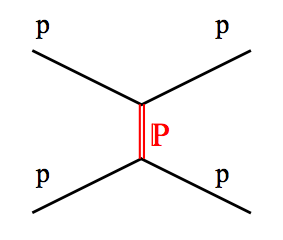
\includegraphics[width=\textwidth]{./Chapters/theory/minimum_bias/images/elastic_scattering.png}
		\caption{Elastic scattering, $p + p \rightarrow p + p$}
		\label{fig: proton-proton interactions - elastic scattering}
	\end{subfigure}
	\begin{subfigure}[h]{0.32\textwidth}
		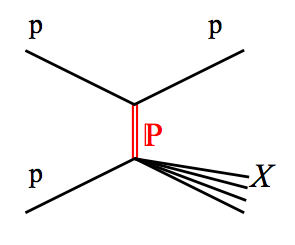
\includegraphics[width=\textwidth]{./Chapters/theory/minimum_bias/images/single_diffractive.png}
		\caption{Single diffractive scattering, $p + p \rightarrow p + X$}
		\label{fig: proton-proton interactions - single diffractive scattering}
	\end{subfigure}
	\begin{subfigure}[h]{0.32\textwidth}
		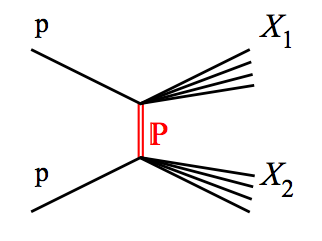
\includegraphics[width=\textwidth]{./Chapters/theory/minimum_bias/images/double_diffractive.png}
		\caption{Double diffractive scattering, $p + p \rightarrow X + X'$}
		\label{fig: proton-proton interactions - double diffractive scattering}
	\end{subfigure}
	\caption{Examples of elastic and inelastic proton-proton interactions via the exchange of a pomeron \cite{Kwiecinski:314736}.}
	\label{fig: elastic and inelastic proton-proton scattering}
\end{figure}

Minimum bias data is dominated by soft QCD physics characterised by low $p_T$ particles and long interaction distances. This property of minimum bias data makes it the ideal region in which to validate, tune and develop phenomenological models e.g. particle production and the structure of the proton. Furthermore minimum bias data is a good approximation of the underlying event (see section \ref{section: underlying event}) which accompanies a hard scale scatter; a good understanding of this translates to a good understanding of the associated hard energy scale physics such as the rare B decays integral to understanding matter and anti-matter physics.
